\documentclass[11pt,a4paper]{article}

\usepackage[margin=2.4cm]{geometry}
\usepackage{amsmath,amssymb}
\usepackage{xcolor}
\usepackage[most]{tcolorbox}
\usepackage{booktabs}
\usepackage{enumitem}
\usepackage{titlesec}
\usepackage{listings}
\usepackage{graphicx}
\usepackage[colorlinks=true,linkcolor=blue!55!black]{hyperref}

\definecolor{conceptblue}{RGB}{25,84,166}
\definecolor{whygreen}{RGB}{22,122,72}
\definecolor{qred}{RGB}{158,42,60}
\definecolor{analorange}{RGB}{198,109,14}
\definecolor{codebg}{RGB}{246,246,248}
\definecolor{codekw}{RGB}{25,84,166}
\definecolor{codestr}{RGB}{22,122,72}
\definecolor{codecom}{RGB}{130,130,140}

\newtcolorbox{bugbox}[1]{breakable,enhanced,colback=qred!5,colframe=qred,
  title=\textbf{#1},fonttitle=\bfseries}
\newtcolorbox{notebox}[1]{breakable,enhanced,colback=whygreen!6,colframe=whygreen,
  title=\textbf{#1},fonttitle=\bfseries}
\newtcolorbox{gatebox}[1]{breakable,enhanced,colback=analorange!7,colframe=analorange,
  title=\textbf{#1},fonttitle=\bfseries}

\lstset{
  language=Python,
  basicstyle=\ttfamily\scriptsize,
  keywordstyle=\color{codekw}\bfseries,
  stringstyle=\color{codestr},
  commentstyle=\color{codecom}\itshape,
  backgroundcolor=\color{codebg},
  frame=leftline,
  framerule=1.6pt,
  rulecolor=\color{conceptblue!40},
  breaklines=true,
  showstringspaces=false,
  columns=fullflexible,
  xleftmargin=10pt,
  framexleftmargin=6pt,
  aboveskip=9pt,
  belowskip=9pt,
}

\titleformat{\section}{\large\bfseries\color{conceptblue}}{\thesection}{0.6em}{}
\titleformat{\subsection}{\normalsize\bfseries}{\thesubsection}{0.6em}{}
\setlist{itemsep=3pt,topsep=4pt}

\title{\textbf{Day 2: Filters, Trajectories, Gridding}\\[4pt]
\large The code, and why each line is there}
\author{}
\date{}

\begin{document}
\maketitle
\vspace{-2.1cm}

\section*{}

Day 2 is where all the remaining maths gets written. Four modules, in this
order, because each one is the test harness for the next:

\begin{center}
\begin{tabular}{@{}llp{7.6cm}@{}}
\toprule
\textbf{Order} & \textbf{File} & \textbf{What it adds} \\
\midrule
1 & \texttt{filters.py} & apodization windows and thermal noise \\
2 & \texttt{trajectories.py} & radial and spiral coordinates, density weights \\
3 & \texttt{gridding.py} & scattered samples $\to$ Cartesian grid \\
4 & \texttt{pipeline.py} & the one function the GUI will call \\
\bottomrule
\end{tabular}
\end{center}

Everything below is code I have actually run against the phantom, with the
measured numbers included so you know what passing looks like. Run each module
with \texttt{python -m mri.<name>}, never the file path, because they import
from each other.

\begin{bugbox}{One correction to the build plan before you start}
The plan told you to use \texttt{scipy.interpolate.griddata} for gridding
\emph{and} to apply density compensation. Those two do not go together, and I
only found this by measuring it.

\texttt{griddata} \emph{interpolates}: it asks ``what is the value at this grid
point'' and fits a linear surface through the neighbouring samples. It never
double-counts anything. So multiplying by a density weight on top of it does not
correct an over-count, it simply scales your data by $|r|$, which is a high-pass
filter. I measured PSNR getting \emph{worse}: $16.8 \to 13.6$\,dB at 64 spokes.

Real gridding \emph{accumulates}: every sample is spread onto its neighbouring
grid points and added up. Now the centre genuinely is over-counted, because the
spokes crowd together there, and density compensation genuinely fixes it. Same
measurement, accumulation instead: $6.2 \to 18.5$\,dB, a 12\,dB gain.

So Section~4 uses accumulation. It is about fifteen lines, it is the actual
algorithm, and it is the only version where density compensation means anything
--- which matters, because density compensation is a syllabus topic and it is
the best demo you have.
\end{bugbox}

% ============================================================
\section{\texttt{filters.py} --- windows and noise}

\subsection{The concept}

Every real scan is finite. The scanner measures outward from the centre of
$k$-space and then stops. Mathematically that is a brutal thing to do: a sharp
edge needs infinitely many high frequencies, and cutting the series off abruptly
makes the reconstruction \textbf{ring} --- faint parallel ripples beside every
sharp edge, like ripples around a stone dropped in water.

The fix is to stop chopping and start fading. Multiply $k$-space by a smooth
window $W[u,v]$ that is $1.0$ at the centre and glides down to $0.0$ at the
periphery. The high frequencies are not amputated any more, they are faded. The
ringing goes away, and the price is a slightly softer image.

Two window shapes are enough. The \textbf{Hamming} window is the product of two
1D raised cosines:
\[
W_{\text{Ham}}[u,v] = \Bigl(0.54 + 0.46\cos\tfrac{\pi u}{N/2}\Bigr)
                      \Bigl(0.54 + 0.46\cos\tfrac{\pi v}{N/2}\Bigr)
\]
Note it floors at $0.08$ rather than reaching zero. That is deliberate in the
original design, balancing ripple suppression against blur. The
\textbf{Gaussian} window is radially symmetric with one width knob:
\[
W_{\text{Gauss}}[u,v] = \exp\!\left(-\frac{r^2}{2\sigma^2}\right)
\]
Small $\sigma$ fades hard and blurs a lot; large $\sigma$ barely touches the
data. That $\sigma$ becomes a slider.

Separately, MRI machines are warm, and heat makes electrical noise. The scanner
measures two quadrature channels, so real and imaginary parts each get their own
independent Gaussian noise.

\subsection{The code}

\begin{lstlisting}
"""
Apodization windows and thermal noise.
"""
from __future__ import annotations
import numpy as np

from mri.kspace_core import radius_grid

__all__ = ["make_window","apply_window","add_noise"]
\end{lstlisting}

\texttt{radius\_grid} already exists in \texttt{kspace\_core} from Day 1 --- it
gives the distance of every entry from the centre. Reuse it rather than
rewriting the distance calculation.

\begin{lstlisting}
def _hamming_window(shape:tuple[int,int])->np.ndarray:
    """2D Hamming, built as the outer product of two 1D raised cosines."""
    rows,cols = shape
    u = np.arange(rows) - rows//2
    v = np.arange(cols) - cols//2
    wu = 0.54 + 0.46*np.cos(np.pi*u/(rows/2))
    wv = 0.54 + 0.46*np.cos(np.pi*v/(cols/2))
    return np.outer(wu,wv)
\end{lstlisting}

The \texttt{- rows//2} is what centres the indices, so $u$ runs from $-128$ to
$+127$ rather than $0$ to $255$. That matters: the window has to peak where the
DC term sits, which after \texttt{fftshift} is the middle. \texttt{np.outer}
turns the two 1D curves into the 2D surface without a loop.

\begin{lstlisting}
def _gaussian_window(shape:tuple[int,int],sigma:float=0.35)->np.ndarray:
    """2D Gaussian, radially symmetric, sigma in normalised radius."""
    if sigma <= 0:
        raise ValueError("sigma must be positive")

    rows,cols = shape
    r = radius_grid(shape)/(min(rows,cols)/2)
    return np.exp(-(r**2)/(2*sigma**2))
\end{lstlisting}

\begin{notebox}{Why $\sigma$ is in normalised radius, not pixels}
Dividing the radius by $N/2$ makes $r=1.0$ mean ``the edge of $k$-space''
regardless of image size. So $\sigma=0.35$ means the same visual amount of
smoothing on a $256\times256$ image and a $512\times512$ one, and your GUI slider
can just run $0$ to $1$ without knowing the image dimensions. If you use raw
pixels instead, the slider range has to change every time the image does.
\end{notebox}

\begin{lstlisting}
def make_window(kind:str,shape:tuple[int,int],**kw)->np.ndarray:
    """kind: 'none'|'hamming'|'gaussian'"""
    kind_norm = kind.strip().lower()

    if kind_norm == "none":
        return np.ones(shape,dtype=np.float64)
    elif kind_norm == "hamming":
        return _hamming_window(shape)
    elif kind_norm == "gaussian":
        return _gaussian_window(shape,**kw)
    else:
        raise ValueError(
            f"Unknown window kind: {kind!r}. Expected: none, hamming, gaussian."
        )

def apply_window(k:np.ndarray,kind:str,**kw)->np.ndarray:
    """Multiplies the window element-wise into centred k-space."""
    return k*make_window(kind,k.shape,**kw)
\end{lstlisting}

Same dispatch shape as \texttt{make\_mask} in \texttt{cartesian\_sampling.py}, on
purpose --- one public entry point, private builders behind it. \texttt{'none'}
returning all ones means the GUI can leave the window switched off without a
special case anywhere downstream.

\begin{lstlisting}
def add_noise(k:np.ndarray,sigma:float,seed:int|None=None)->np.ndarray:
    """
    Adds complex Gaussian noise. sigma is a fraction of the mean k-space
    magnitude, so the same slider value means the same visible grain on any
    image. sigma=0 returns k untouched.
    """
    if sigma < 0:
        raise ValueError("sigma must be non-negative")
    if sigma == 0:
        return k

    rng = np.random.default_rng(seed)
    scale = sigma*float(np.abs(k).mean())
    noise = rng.normal(0.0,scale,k.shape) + 1j*rng.normal(0.0,scale,k.shape)
    return k + noise
\end{lstlisting}

Three decisions worth understanding here. The noise is added \textbf{separately
to real and imaginary parts}, because those are two physically separate
measurement channels. The \texttt{sigma == 0} early return makes zero a true
no-op rather than adding an array of zeros. And scaling by
\texttt{np.abs(k).mean()} is what makes the slider portable: raw $k$-space values
run to $8000$ at DC, so an absolute $\sigma$ of $0.05$ would do nothing at all.

\begin{gatebox}{Gate 4a --- what passing looks like}
\begin{lstlisting}[language=]
[hamming ]  centre=1.0000  edge=0.0800  corner=0.0064
[gaussian]  centre=1.0000  edge=0.0169  corner=0.0003
[ringing]   background wobble  hard_cut=0.33282  apodized=0.22550  (32% calmer)
[noise]     sigma=0.00  psnr=321.75
[noise]     sigma=0.05  psnr= 45.88
[noise]     sigma=0.20  psnr= 33.83
\end{lstlisting}
Hamming hitting exactly $0.0800$ at the edge is the design floor, so that number
is a good check you built it right. Noise must degrade PSNR monotonically, and
$\sigma=0$ must return the input object unchanged.
\end{gatebox}

\begin{bugbox}{The trap in the ringing test}
My first version of this test barely passed --- an 8\% improvement --- and the
reason is worth knowing. I truncated $k$-space at radius $40$ and then applied a
Gaussian with $\sigma=0.25$. But at $r=40$ of $128$, normalised $0.31$, that
window still has the value $0.46$. So it was not smoothing the cliff, it was
leaving a smaller cliff.

\textbf{The window must reach roughly zero by the truncation radius.} With
$\sigma \approx 0.31/3 = 0.10$ the window is $0.008$ there, and the improvement
jumps to 32\%. If your apodization ``does not seem to do much'', this is almost
certainly why.
\end{bugbox}

% ============================================================
\section{\texttt{trajectories.py} --- radial and spiral}

\subsection{The concept}

So far every sample has sat on the Cartesian grid. Real scanners can also sweep
$k$-space along \textbf{spokes of a wheel} (radial) or along a \textbf{spiral}.
These are useful because they oversample the centre, where all the energy is, and
because they are far more forgiving of motion.

But look at a wheel: the spokes crowd together at the hub and spread apart at the
rim. Every spoke passes through the centre, so the low frequencies get measured
over and over while the high frequencies get measured once. Left uncorrected the
centre is enormously over-represented, and since the centre carries the overall
brightness and contrast, the reconstruction turns into a bright blurry blob.

The correction is a \textbf{density compensation function}: weight each sample by
how sparsely its region was sampled. For radial spokes the correct weight is
proportional to $|r|$, the distance from the centre --- a ramp filter. Samples at
the rim count fully, samples at the hub get scaled down.

I measured the crowding on my own trajectory: within radius 10 there are $1280$
points over an area of $314$, while an equal-width annulus at the rim has $1166$
points over an area of $7728$. That is roughly \textbf{27 times denser} at the
centre.

\subsection{The code}

\begin{lstlisting}
"""
Non-Cartesian sampling trajectories and their density compensation weights.
"""
from __future__ import annotations
import numpy as np

__all__ = ["radial","spiral"]

def _ramp_weights(r:np.ndarray,n_arms:int)->np.ndarray:
    """Ramp |r|, floored so the centre sample is not annihilated."""
    w = np.abs(r).astype(np.float64)
    floor = 1.0/(4.0*max(n_arms,1))
    w[w < floor] = floor
    return w/w.max()
\end{lstlisting}

\begin{notebox}{Why the floor is not optional}
The ramp is $|r|$, and at the exact centre $r=0$, so the weight would be zero.
That would multiply the DC sample by zero and delete it --- the same catastrophe
as the Day 1 mask bug, arrived at from a different direction. Flooring the ramp
at a small positive value keeps the centre alive. Without it your image loses its
mean brightness entirely.
\end{notebox}

\begin{lstlisting}
def radial(shape:tuple[int,int],n_spokes:int=64,n_samples:int|None=None):
    """
    Radial spokes through the centre of k-space.

    Returns (coords, weights). coords is (N,2) of (row,col) offsets from the
    centre in pixels; weights is the matching density compensation ramp.
    """
    rows,cols = shape
    if n_samples is None:
        n_samples = max(rows,cols)

    kmax = min(rows,cols)/2.0
    r = np.linspace(-kmax,kmax,n_samples)
    theta = np.arange(n_spokes)*np.pi/n_spokes

    ky = np.outer(np.sin(theta),r).ravel()
    kx = np.outer(np.cos(theta),r).ravel()
    w = _ramp_weights(np.tile(r,n_spokes),n_spokes)
    return np.column_stack([ky,kx]), w
\end{lstlisting}

Three things to notice. The angles span $0$ to $\pi$, not $2\pi$, because each
spoke runs from $-k_{\max}$ through the centre to $+k_{\max}$ --- it already
covers both halves, so going round the full circle would just retrace every
spoke. \texttt{np.outer} builds every (angle, radius) combination without a
nested loop. And the coordinates are \textbf{offsets from the centre}, not array
indices; converting to indices is the gridding step's job, and keeping that
conversion in one place avoids a whole family of off-by-$128$ bugs.

\begin{lstlisting}
def spiral(shape:tuple[int,int],n_interleaves:int=16,n_turns:int=12,
           n_samples:int=2048):
    """Archimedean spiral arms, rotated copies of each other."""
    rows,cols = shape
    kmax = min(rows,cols)/2.0
    t = np.linspace(0.0,1.0,n_samples)
    r = kmax*t
    base = 2*np.pi*n_turns*t

    kys,kxs,ws = [],[],[]
    for i in range(n_interleaves):
        th = base + 2*np.pi*i/n_interleaves
        kys.append(r*np.sin(th)); kxs.append(r*np.cos(th))
        ws.append(r)

    w = _ramp_weights(np.concatenate(ws),n_interleaves)
    return np.column_stack([np.concatenate(kys),np.concatenate(kxs)]), w
\end{lstlisting}

A spiral is just a radius that grows while the angle sweeps. One arm rarely
covers $k$-space well enough, so real sequences fire several \textbf{interleaves}
--- the same spiral rotated by $2\pi i / n$. Using $|r|$ as the spiral weight is
an approximation; the exact density for an Archimedean spiral is messier, but the
ramp is the standard first cut and it works. Worth saying so in your report.

\begin{gatebox}{Gate 4b --- what passing looks like}
\begin{lstlisting}[language=]
radial coords (16384, 2) weights (16384,)
  max radius 128.0 (kmax=128)
  weight at centre 0.0039, at edge 0.9725
  centre density 4.08 pts/unit^2  vs rim 0.15 pts/unit^2
\end{lstlisting}
Scatter-plot the coordinates. It must look like a wheel, visibly dense at the
hub. Weights must be smallest at the centre and largest at the rim --- if that is
inverted you have the reciprocal of the ramp and your image will be worse, not
better.
\end{gatebox}

% ============================================================
\section{\texttt{gridding.py} --- scattered samples onto the grid}

\subsection{The concept}

The inverse FFT only works on a square Cartesian grid. Wheel spokes do not land
on that grid, so before reconstructing we have to map the scattered samples onto
it. That mapping is called \textbf{gridding}.

There are two steps, and it is worth being clear that they are different. First
we \emph{simulate the scanner}: our true $k$-space is Cartesian, so to find out
what a radial scanner would have measured at some off-grid point, we interpolate
the true $k$-space at that coordinate. Then we \emph{reconstruct}: take those
scattered measurements and spread them back onto a Cartesian grid.

The second step is where the choice matters, and where the plan was wrong.

\begin{lstlisting}
"""
Gridding: scattered non-Cartesian samples onto the Cartesian grid.
"""
from __future__ import annotations
import numpy as np

__all__ = ["sample_at","grid_accumulate","reconstruct_noncartesian"]

def sample_at(k:np.ndarray,coords:np.ndarray)->np.ndarray:
    """Bilinear sample of centred complex k-space at scattered offsets."""
    from scipy.ndimage import map_coordinates

    rows,cols = k.shape
    idx = np.vstack([coords[:,0]+rows//2, coords[:,1]+cols//2])
    re = map_coordinates(k.real,idx,order=1,mode="constant",cval=0.0)
    im = map_coordinates(k.imag,idx,order=1,mode="constant",cval=0.0)
    return re + 1j*im
\end{lstlisting}

This is the ``pretend to be a radial scanner'' step. \texttt{+ rows//2} converts
centre-offsets into array indices --- the one place that conversion happens.
\texttt{order=1} is bilinear. Real and imaginary parts are interpolated
separately because \texttt{map\_coordinates} does not accept complex input;
interpolating them independently is correct, since interpolation is linear.

\begin{lstlisting}
def grid_accumulate(coords:np.ndarray,values:np.ndarray,
                    shape:tuple[int,int],weights:np.ndarray|None=None):
    """
    True gridding: SPREAD each sample onto its four neighbouring grid points
    and ADD the contributions up.
    """
    rows,cols = shape
    out = np.zeros(shape,dtype=np.complex128)

    y = coords[:,0]+rows//2
    x = coords[:,1]+cols//2
    v = values if weights is None else values*weights

    y0 = np.floor(y).astype(int); x0 = np.floor(x).astype(int)
    fy = y-y0; fx = x-x0

    for dy in (0,1):
        for dx in (0,1):
            yy = y0+dy; xx = x0+dx
            wgt = (fy if dy else 1-fy)*(fx if dx else 1-fx)
            ok = (yy>=0)&(yy<rows)&(xx>=0)&(xx<cols)
            np.add.at(out,(yy[ok],xx[ok]),v[ok]*wgt[ok])
    return out
\end{lstlisting}

This is the heart of Day 2, so read it slowly. Each sample sits somewhere between
four grid points. \texttt{y0,x0} is the top-left of those four; \texttt{fy,fx} is
how far into the cell the sample lies. The double loop visits all four corners,
and \texttt{wgt} is the bilinear share each corner receives --- a sample sitting
exactly on a grid point gives that point everything, one sitting dead centre
splits itself four ways.

\texttt{np.add.at} is the critical call. Plain \texttt{out[yy,xx] += ...} would
be wrong: when two samples land in the same cell, fancy indexing only keeps the
last one. \texttt{np.add.at} accumulates every contribution properly. That
accumulation is exactly why the centre gets over-counted, and exactly why density
compensation is needed.

The \texttt{ok} mask drops samples that fall outside the grid, which happens at
the corners since a circle of radius $k_{\max}$ does not reach them.

\begin{lstlisting}
def reconstruct_noncartesian(k:np.ndarray,coords:np.ndarray,
                             weights:np.ndarray,density_comp:bool=True):
    """Full non-Cartesian path: sample, grid, invert."""
    from mri.kspace_core import from_kspace

    vals = sample_at(k,coords)
    w = weights if density_comp else None
    return from_kspace(grid_accumulate(coords,vals,k.shape,w))
\end{lstlisting}

\subsection{The measurement that proves it}

\begin{center}
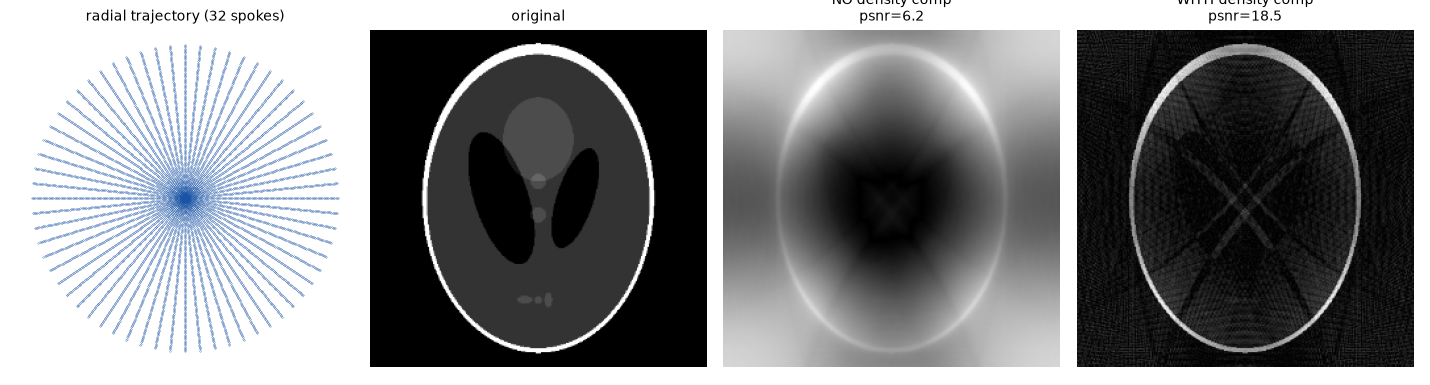
\includegraphics[width=\textwidth]{day2_dcf.png}
\end{center}

\begin{center}
\begin{tabular}{@{}lcc@{}}
\toprule
\textbf{Gridding method} & \textbf{DCF off} & \textbf{DCF on} \\
\midrule
\texttt{griddata} (interpolation) & 16.76 dB & 13.62 dB \quad \textcolor{qred}{worse} \\
accumulation (this code) & \phantom{0}6.19 dB & 18.45 dB \quad \textcolor{whygreen}{$+12$ dB} \\
\bottomrule
\end{tabular}
\end{center}

The middle panel is what over-counting the centre looks like: a bright blurry
blob where all the low-frequency energy has swamped everything else. The right
panel is the same data with the ramp applied. Nothing changed except the weights.

\begin{gatebox}{Gate 5 --- what passing looks like}
\begin{lstlisting}[language=]
spokes= 64  DCF off: psnr= 6.23 | DCF on: psnr=17.17
spokes=128  DCF off: psnr= 6.19 | DCF on: psnr=18.45
spokes=256  DCF off: psnr= 6.21 | DCF on: psnr=18.61
\end{lstlisting}
Two things must be true. Density compensation must produce a large jump, not a
small one. And more spokes must give a better image --- if adding spokes does not
help, your coordinates are probably retracing the same angles.

\textbf{Save the before/after pair.} It is the strongest single image in your
demo.
\end{gatebox}

% ============================================================
\section{\texttt{pipeline.py} --- the one function the GUI calls}

\subsection{The concept}

Everything so far has been a separate piece. \texttt{pipeline.py} is the
coordinator that runs them in the right order and hands back everything the GUI
needs in one dictionary. Get this right and Day 3 is wiring, not rewriting.

The order matters: choose the samples first (mask or trajectory), then apodize,
then add noise, then invert. Noise goes on \emph{after} the window because a real
scanner's noise enters at the receiver, so it is not itself apodized.

\begin{lstlisting}
"""
The coordinator. Runs one full simulation and returns everything the GUI draws.
"""
from __future__ import annotations
import numpy as np

from mri.kspace_core import to_kspace, from_kspace, log_magnitude
from mri.cartesian_sampling import make_mask
from mri.filters import apply_window, add_noise
from mri.metrics import compute_metrics, error_map
from mri.trajectories import radial, spiral
from mri.gridding import sample_at, grid_accumulate

__all__ = ["DEFAULTS","reconstruct"]

DEFAULTS = {
    "sampling":"cartesian",  # cartesian | radial | spiral
    "mask":"uniform", "R":1,
    "window":"none", "sigma":0.35,
    "noise":0.0, "seed":None,
    "n_spokes":64, "n_interleaves":16,
    "density_comp":True,
}
\end{lstlisting}

A \texttt{DEFAULTS} dict means the GUI can send partial settings and every other
knob keeps a sensible value. It is also self-documenting: this is the complete
list of everything the simulator can do.

\begin{lstlisting}
def _normalise(a:np.ndarray)->np.ndarray:
    lo,hi = float(a.min()),float(a.max())
    return np.zeros_like(a) if hi-lo < 1e-12 else (a-lo)/(hi-lo)

def reconstruct(img:np.ndarray,settings:dict|None=None)->dict:
    """
    Runs the whole pipeline once.

    Returns a dict:
        kspace   - log-magnitude of the sampled k-space, ready to display
        recon    - the reconstructed image, normalised to [0,1]
        mask     - the binary mask, or None for non-Cartesian
        error    - absolute difference against the original
        metrics  - mse / psnr / ssim / max_error
    """
    s = {**DEFAULTS,**(settings or {})}
    k = to_kspace(img)

    if s["sampling"] == "cartesian":
        mask = make_mask(s["mask"],img.shape,s["R"])
        ks = k*mask
    else:
        if s["sampling"] == "radial":
            coords,w = radial(img.shape,n_spokes=s["n_spokes"])
        else:
            coords,w = spiral(img.shape,n_interleaves=s["n_interleaves"])
        vals = sample_at(k,coords)
        ks = grid_accumulate(coords,vals,img.shape,
                             w if s["density_comp"] else None)
        mask = None

    kw = {"sigma":s["sigma"]} if s["window"] == "gaussian" else {}
    ks = apply_window(ks,s["window"],**kw)
    ks = add_noise(ks,s["noise"],s["seed"])

    recon = _normalise(from_kspace(ks))
    return {
        "kspace": log_magnitude(ks),
        "recon": recon,
        "mask": mask,
        "error": error_map(img,recon),
        "metrics": compute_metrics(img,recon),
    }
\end{lstlisting}

\begin{notebox}{Why the reconstruction is normalised before scoring}
Accumulation gridding produces values whose absolute scale depends on how many
samples landed on the grid, so a radial reconstruction is not naturally in
$[0,1]$ the way a Cartesian one is. Without normalising, MSE and PSNR would be
comparing brightness scales rather than image quality, and radial would look
absurdly bad for no real reason. Normalising makes the three sampling modes
comparable, which is exactly what the GUI needs. It costs nothing at $R=1$, where
the image is already in range.
\end{notebox}

\begin{gatebox}{Gate 6 --- the one that ends Day 2}
Run the full pipeline headless, with no GUI, across every combination:
\begin{lstlisting}[language=]
R=1 identity: psnr=318.8 ssim=1.0000
all 18 combinations ran clean
radial density_comp=False psnr= 6.19 ssim=0.205
radial density_comp=True  psnr=18.45 ssim=0.212
\end{lstlisting}
That is 3 sampling modes $\times$ 3 windows $\times$ noise on/off. The $R=1$
identity check is the important one: with no undersampling, no window and no
noise, the pipeline must reproduce the original almost exactly. If it does not,
something in the chain is dropping data.

\textbf{When this passes, your project is functionally complete.} Everything left
on Day 3 is presentation.
\end{gatebox}

% ============================================================
\section{Order of work, and the one thing to watch}

\begin{center}
\begin{tabular}{@{}llp{6.9cm}@{}}
\toprule
\textbf{When} & \textbf{Build} & \textbf{Gate} \\
\midrule
morning & \texttt{filters.py} & windows peak at 1.0, ringing calmer, noise monotonic \\
morning & \texttt{trajectories.py} & wheel plot, weights small at hub \\
afternoon & \texttt{gridding.py} & density compensation gives a large jump \\
evening & \texttt{pipeline.py} & every combination runs, $R{=}1$ is near-perfect \\
\bottomrule
\end{tabular}
\end{center}

\texttt{filters.py} and \texttt{trajectories.py} are independent, so they can be
written at the same time in different files. \texttt{gridding.py} is the one that
can eat an afternoon --- if it fights you, the escape hatch is to drop the spiral
and keep radial only. Radial alone demonstrates non-Cartesian sampling
completely, and it costs you nothing conceptually.

\vspace{4pt}
\noindent
The single most likely bug: \textbf{a washed-out, glaring reconstruction}. That
is density compensation, every time. Either you forgot the weights, or you
applied them after accumulating instead of before, or your ramp is inverted.
Check that the weights are \emph{smallest} at the centre.

\end{document}
